\section{Apêndice A – Sistema Operacional}
\label{apendeceA}

Além do trabalho desenvolvido no projeto, um protótipo de sistema operacional foi feito.

Esse protótipo contempla: inicialização.

 Conteúdos que foram compreendidos a partir do desenvolvimento de um \href{https://github.com/gzsig/zsig-OS}{sistema operacional} simples que passa por todas as etapas essenciais do processo de ``boot'' – ilustrado na figura a baixo – \textit{state-of-the-art} de computadores clássicos: ligando em `modo real de 16 bits', carregando o kernel\footnote{Uma parte integrante de qualquer sistema operacional. Que se constitui em um programa com controle completo sobre tudo no sistema.}, transferindo-se para `modo protegido de 32 bits' e `gerenciando interrupções'.

\vspace{1cm}
\begin{figure}[H] \centering 
  \makebox[\textwidth][c]{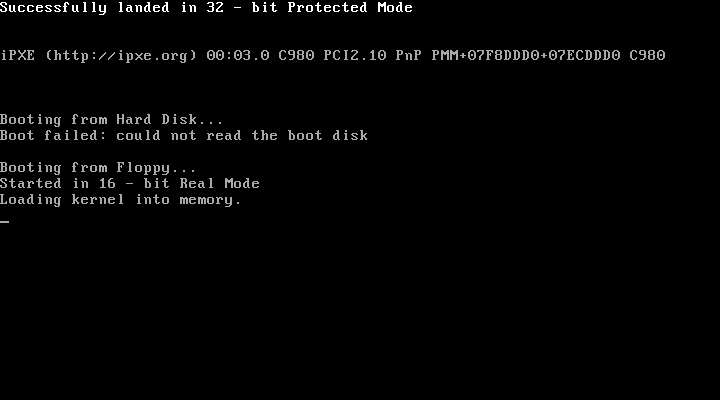
\includegraphics[width=0.8\textwidth]{zsig_OS_boot.png}}
  \caption{\label{zsig_OS_boot} Processo de boot} 
\end{figure}
